\documentclass{beamer}
\usepackage[czech]{babel}
\usepackage[utf8]{inputenc}
\usepackage{picture}
\usetheme{Pittsburgh}
\title{Vytváření dopředné neuronové sítě pomocí algoritmu Tiling}
\institute{FIT VUT v Brně}
\author{Jan Sedlák}
\date{2013}
\begin{document}

\begin{frame}
  \maketitle
\end{frame}

\begin{frame}{Algoritmus Tiling}
  Dynamické vytváření neuronové sítě:
  \begin{itemize}
    \item klasifikace pouze do dvou skupin,
    \item používá perceptrony,
    \item pro učení pocket algoritmus,
    \item v každé vrstvě musí dosáhnout ``věrohodnosti''.
  \end{itemize}
\end{frame}

\begin{frame}{Princip fungování}
\begin{columns}
  \begin{column}{0.47\textwidth}
    \begin{itemize}
    \item První neuron je Master:
      \begin{itemize}
      \item snaží se co nejlépe klasifikovat vstup,
      \item algoritmus končí vytvořením posledního Master neuronu.
      \end{itemize}
    \item Další neurony ve vrstvě jsou Ancillary:
      \begin{itemize}
      \item snaží se zaručit věrohodnost vrstvy.
      \end{itemize}
    \end{itemize}
  \end{column}
  \begin{column}{0.5\textwidth}
    \includegraphics[width=\textwidth]{nn.eps}
  \end{column}
\end{columns}
\end{frame}

\begin{frame}{Problém s pocket algoritmem}
  \begin{figure}
    \centering
    \setlength{\unitlength}{1.5cm}
    \begin{picture}(4, 4)
      \put(0,2){\line(1,0){4}}
      \put(2,0){\line(0,1){4}}
      \put(3.8,1.8){$x_1$}
      \put(2.2,3.8){$x_2$}
      \put(1,3){\circle*{0.2}}
      \put(2,3){\circle*{0.2}}
      \put(3,3){\circle*{0.2}}
      \put(1,2){\circle*{0.2}}
      \put(2,2){\circle{0.2}}
      \put(3,2){\circle*{0.2}}
      \put(1,1){\circle*{0.2}}
      \put(2,1){\circle*{0.2}}
      \put(3,1){\circle*{0.2}}
      \put(0,0){\line(4,1){4}}
      \put(3.8,0.7){$S$}
    \end{picture}
  \end{figure}
\end{frame}

\begin{frame}{Praktická úloha}
  \begin{columns}
    \begin{column}{0.47\textwidth}
      \begin{itemize}
      \item desetinásobná stratifikovaná ten-fold křížová validace
      \item Iris dataset
        \begin{itemize}
        \item odebrána lineárně separovatelná třída
        \item úspěšnost kolem 94{,}5 \%
        \end{itemize}
      \item funkce sudosti počtu jedniček na vstupu
        \begin{itemize}
        \item úspěšnost 41{,}8 \%
        \end{itemize}
      \end{itemize}
    \end{column}
    \begin{column}{0.5\textwidth}
      \includegraphics[width=\textwidth]{iris.png}
    \end{column}
  \end{columns}
\end{frame}

\end{document}
